\chapter{General theory of bisimulations and unfoldings in accessible categories}
\label{chap:bisunf}

In this chapter, I would like to come back to the general theory of bisimulations from \cite{joyal96}, presented in Chapter 1 in the case of transition systems. This chapter is not directly related to the rest of this thesis. No particular focus on true concurrency or geometry will be made (although we will talk about the universal covering of a groupoid), and this chapter may be skipped for a first reading.

In Chapter 1, we have seen that the general idea was to provide conditions on morphisms of systems for them to act like bisimulations. We saw that the main point was that such morphisms must lift executions. In the original paper \cite{joyal96}, this general idea was formalized: as long as you provide a category of models and a sub-category of ``path shapes'' (for example, branches in the case of transition systems), it is possible to describe a notion of bisimilarity as the existence of a span of morphisms that lifts executions. A number of occurrences of this theory can be observed: transition systems with bisimulations, transition systems with independence and (strong) history-preserving bisimulations, ... can be describe as such. Also in this paper, another general theory of bisimulations, more classic, was described: two systems are bisimilar if there is a relation between their executions. Those two theories were proved to coincide with classical theory of bisimulations, but there were no general results stating that both theories coincide generally.

Independently, we have seen that unfoldings are important for computational systems. They allow one to consider systems which are simpler since they do not have any looping behaviors. Theoretically, the unfolding process is in general a right adjoint of some inclusion of ``simple systems'' into the full category of systems, for example, inclusion of synchronization trees into transition systems, or event structures into transition systems with independence.

In this chapter, we describe a general class of systems, called \textbf{accessible categorical models}, with specified path shapes that satisfies some conditions, intuitively, that we can form trees from path shapes. In this general theory, both theories of bisimulations from \cite{joyal96} coincide and a nice notion of unfolding can be described. In Section 1, we recall the general theory from \cite{joyal96} and in Section 2, we describe accessible categorical models by explaining why in this case both theories of bisimulations coincide. We then prove that presheaf models from \cite{joyal96} are accessible (Section 3) and that accessibility is preserved by coreflections (Section 4). In Section 5, we describe the general definition of unfoldings and show that this produces a bisimilar system and that unfolding is the right adjoint of some inclusion. Finally, in Section 6, following intuitions from universal coverings from algebraic topology, we prove that unfolding is universal, and that the universal covering of a pointed connected groupoid is a particular case of unfolding.




\section{Categorical models and bisimilarities}
\label{catmod}

We first recall, from \cite{joyal96}, two notions of bisimilarities in a category with a specified subcategory of path shapes.


%%%%%%%%%%%%%%%%%%%%%%%%%%%%%%%

\subsection{Category of models, subcategory of paths}

We consider a category $\M$ (of \textbf{models}) together with a small subcategory (of \textbf{path-shapes}) $\PP$. We assume that $\M$ and $\PP$ have a common initial object $I$, i.e., an object $I \in \PP$ such that for every object $A$ of $\PP$ (resp. of $\M$), there is a unique morphism in $\PP$ (resp. in $\M$) from $I$ to $A$. We denote this morphism by $\iota_A$ this unique morphism. One typical example is the category of transition systems $\tr$ together with the subcategory of  branches $\br$. A common initial object of $\tr$ and $\br$ is then the branch of length $0$ $(\textbf{[0]},0,\varnothing)$.




%%%%%%%%%%%%%%%%%%%%%%%%%%%%%%%%%%%%%%%%



\subsection{A relational bisimilarity of models: path-bisimilarity}


Equivalence of transition systems is defined through the notion of \textbf{bisimulation}. Classically, a bisimulation is defined as presented in Section \ref{subsec:bire}, as relation on states.

A bisimulation $R$ between $T_1$ and $T_2$ induces a relation $R_n'$ between executions of length $n$ of $T_1$ and $T_2$ by:
$$R_n' = \{(\map{f_1}{B_1}{T_1},\map{f_2}{B_2}{T_2}) \mid \forall i \in [n], \, (f_1(i),f_2(i)) \in R\}$$
These relations satisfy that:
\begin{itemize}
	\item $(\iota_{T_1},\iota_{T_2}) \in R'_0$ by the first condition of a bisimulation;
	\item by the second condition, if $(f_1,f_2) \in R'_n$ and if $(f_1(n), a, q_1)\in \Delta_1$ then there is $q_2 \in Q_2$ such that $(f_2(n), a, q_2)\in \Delta_2$ and $(f_1',f_2') \in R'_{n+1}$ where $f_i'(j) = f_i(j)$ if $j \leq n$, $q_i$ otherwise;
	\item symmetrically with the third;
	\item if $(f_1,f_2) \in R'_{n+1}$ then $(f'_1,f'_2) \in R'_n$ where $f'_i$ is the restriction of $f_i$ to $[n]$.
\end{itemize}

In fact, bisimilarity of transition systems is equivalent to the existence of such relations on executions. This leads us to the general notion of strong path-bisimulation \cite{joyal96}.

A \textbf{strong path-bisimulation} $R$ between $X$ and $Y$, objects of $\M$ is a set of elements of the form $\pspan{P}{X}{Y}{f}{g}$
	with $P$ an object of $\PP$ such that:
	\begin{itemize}
		\item[(a)] $\pspan{I}{X}{Y}{i_X}{i_Y}$ belongs to $R$;
		\item[(b)] if $\pspan{P}{X}{Y}{f}{g}$ belongs to $R$ then for every \textbf{path extension} of $X$, i.e, every morphism $p$ in $\PP$ such that:
	\begin{center}
		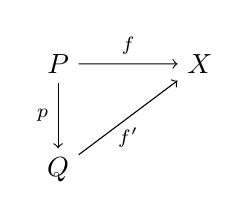
\begin{tikzpicture}[scale=1.5]
		\node (A) at (0,0.9) {$P$};
		\node (B) at (1.2,0.9) {$X$};
		\node (C) at (0,0) {$Q$};
		\path[->,font=\scriptsize]
		(A) edge node[left]{$p$} (C)
		(C) edge node[below]{$f'$} (B)
		(A) edge node[above]{$f$} (B);
	\end{tikzpicture}
	\end{center}
	commutes then there exists a path extension of $Y$
	\begin{center}
		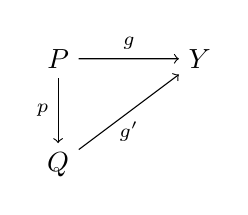
\begin{tikzpicture}[scale=1.5]
		\node (A) at (0,0.9) {$P$};
		\node (B) at (1.2,0.9) {$Y$};
		\node (C) at (0,0) {$Q$};
		\path[->,font=\scriptsize]
		(A) edge node[left]{$p$} (C)
		(C) edge node[below]{$g'$} (B)
		(A) edge node[above]{$g$} (B);
	\end{tikzpicture}
	\end{center}
	such that $\pspan{Q}{X}{Y}{f'}{g'}$ belongs to $R$;
		\item[(c)] symmetrically;
		\item[(d)] if $\pspan{P}{X}{Y}{f}{g}$ belongs to $R$ and if we have a morphism $\map{p}{Q}{P} \in \PP$ then $\pspan{Q}{X}{Y}{f\circ p}{g\circ p}$ belongs to $R$;
	\end{itemize}
We say that $X$ and $Y$ are \textbf{strong path bisimilar} iff there exists a strong path bisimulation between them.







%%%%%%%%%%%%%%%%%%%%%%%%%%%%%%%%%%%


\subsection{A fibrational bisimilarity of models: $\PP$-bisimilarity}

We have seen that in the case of transition systems, bisimilarity is equivalent to the existence of morphisms having lifting properties with respect to executions. This can be extended to any category of models with a specified sub-category of path-shapes.

We say that a morphism $\map{f}{X}{Y}$ of $\M$ is \textbf{($\PP$-)open} iff for every commutative diagram:
	\begin{center}
	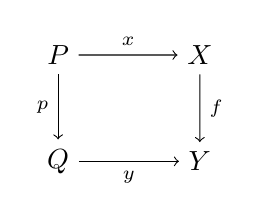
\begin{tikzpicture}[scale=1.5]
		\node (A) at (0,0.9) {$P$};
		\node (B) at (1.2,0.9) {$X$};
		\node (C) at (0,0) {$Q$};
		\node (D) at (1.2,0) {$Y$};
		\path[->,font=\scriptsize]
		(A) edge node[above]{$x$} (B)
		(B) edge node[right]{$f$} (D)
		(C) edge node[below]{$y$} (D)
		(A) edge node[left]{$p$} (C);
	\end{tikzpicture}
	\end{center}
	with $\map{p}{P}{Q} \in \PP$, there exists a morphism $\map{\theta}{Q}{X}$ such that the following diagram commutes:
	\begin{center}
	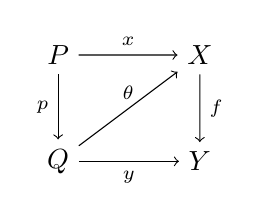
\begin{tikzpicture}[scale=1.5]
		\node (A) at (0,0.9) {$P$};
		\node (B) at (1.2,0.9) {$X$};
		\node (C) at (0,0) {$Q$};
		\node (D) at (1.2,0) {$Y$};
		\path[->,font=\scriptsize]
		(A) edge node[above]{$x$} (B)
		(B) edge node[right]{$f$} (D)
		(C) edge node[below]{$y$} (D)
		(A) edge node[left]{$p$} (C)
		(C) edge node[above]{$\theta$} (B);
	\end{tikzpicture}
	\end{center}
We then say that two objects $X$ and $Y$ of $\M$ are \textbf{$\PP$-bisimilar} iff there exists a span $\map{f}{Z}{X}$ and $\map{g}{Z}{Y}$ where $f$ and $g$ are $\PP$-opens.


It is known that if $X$ and $Y$ are $\PP$-bisimilar then they are strong path bisimilar \cite{joyal96}, but 
the converse does not seem to hold in general. It will hold in the case of transition systems (both $\PP$ and path bisimilarities  coincide with the classical bisimilarity), but there is no general result for the converse. The purpose of the next section is to investigate a general framework in which those two notions of bisimilarities coincide.









%%%%%%%%%%%%%%%%%%%%%%%%%%%%%%%%%
%%%%%%%%%%%%%%%%%%%%%%%%%%%%%%%%%%
%%%%%%%%%%%%%%%%%%%%%%%%%%%%%%%%%







\section{Accessible models and equivalence of bisimilarities}
\label{accmod}



For the converse, we must build a span of open maps from a strong path-bisimulation. It requires in particular that we construct an object of $\M$, which will be the tip of the span. One way of doing so is to glue the elements of the bisimulation in order to obtain an "object of bisimilar paths". Categorically, a glueing is a colimit, so a natural hypothesis should be the existence of some colimits in $\M$.

Concretely, a \textbf{$\PP$-tree} in $\M$ is a colimit in $\M$ of a small diagram with values in $\PP$, i.e., of a functor $\map{D}{\D}{\PP}$ where $\D$ is a small category. We say that \textbf{all $\PP$-trees exist in $\M$} if every small diagram with values in $\PP$ has a colimit in $\M$. In the category of transition systems, $\br$-trees are exactly synchronization trees. In particular, all $\br$-trees exists in $\tr$.
We denote by $\tre{\M}{\PP}$ for the full subcategory of $\M$ of $\PP$-trees.


Let $R$ be a strong path bisimulation between $X$ and $Y$ and assume that all $\PP$-trees exist. Let us construct a span of maps between $X$ and $Y$.
First, we construct the tip of the span as the colimit of a particular diagram with values in $\PP$, defined from $R$. Let $\C$ be the following category:
		\begin{itemize}
			\item objects of $\C$ are elements of $R$;
			\item morphisms from $\pspan{P}{X}{Y}{x}{y}$ to $\pspan{Q}{X}{Y}{x'}{y'}$ are morphisms $\map{p}{P}{Q}$ of $\PP$ such that the following diagram commutes:
				\begin{center}
		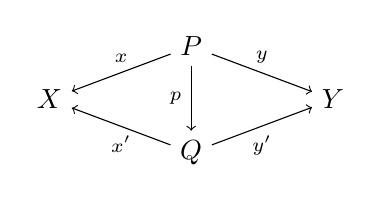
\begin{tikzpicture}[scale=1.5]
		\node (A) at (0,0.9) {$P$};
		\node (B) at (1.2,0.45) {$Y$};
		\node (D) at (-1.2,0.45) {$X$};
		\node (C) at (0,0) {$Q$};
		\path[->,font=\scriptsize]
		(C) edge node[below]{$x'$} (D)
		(A) edge node[above]{$x$} (D)
		(A) edge node[left]{$p$} (C)
		(C) edge node[below]{$y'$} (B)
		(A) edge node[above]{$y$} (B);
	\end{tikzpicture}
	\end{center}
		\end{itemize}
		Then define the diagram $\map{F}{\C}{\PP}$ which maps every $\pspan{P}{X}{Y}{x}{y} \in R$ to $P$ and every $p$ to itself. Since $\PP$-trees exist ($F$ is small because $R$ is a set), let $(Z, ([\alpha])_{\alpha \in R})$ be the colimit of $F$, where the $\map{[\pspan{P}{X}{Y}{x}{y}]}{P = F(\pspan{P}{X}{Y}{x}{y})}{Z}$ are the maps from the colimit.
		
$Z$ will be the tip of our span. Now we need to construct maps $\map{\Phi}{Z}{X}$ and $\map{\Psi}{Z}{Y}$. Let us do it for $\Phi$: since $(X,(F(\pspan{P}{X}{Y}{x}{y}) \xrightarrow{x} X))$ is a cocone of $F$, there exists a unique morphism $\map{\Phi}{Z}{X}$ such that for every $\pspan{P}{X}{Y}{x}{y} \in R$ the following diagram commutes:
		\begin{center}
		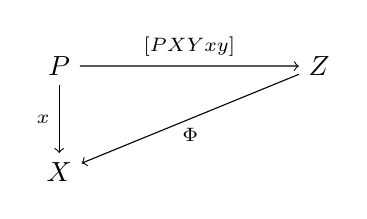
\begin{tikzpicture}[scale=1.5]
		\node (A) at (0,0.9) {$P$};
		\node (B) at (2.2,0.9) {$Z$};
		\node (C) at (0,0) {$X$};
		\path[->,font=\scriptsize]
		(A) edge node[left]{$x$} (C)
		(B) edge node[below]{$\Phi$} (C)
		(A) edge node[above]{$[\pspan{P}{X}{Y}{x}{y}]$} (B);
	\end{tikzpicture}
	\end{center}
	
To prove that strong path-bisimilarity implies $\PP$-bisimilarity, we just need to prove that $\Phi$ is open, but this does not hold in general. 
We will need that we do not create more paths in a tree than the ones we used in the glueing. In the case of transition systems, this says that every path in a tree seen as the colimit of a certain diagram $D$ with values in $\br$ is a subbranch of some $D(i)$. More generally, we will say that $\M$ is \textbf{$\PP$-accessible} if:
\begin{itemize}
	\item all $\PP$-trees exist;
	\item every morphism $\map{f}{P}{Z}$ where $P \in \PP$ and $(Z,(\eta_d)_{d\in\D})$ is the colimit of a non-empty small diagram $\map{D}{\D}{\PP}$ factorizes as $f = \eta_d\circ p$ for some $d \in \D$ with $\map{p}{P}{D(d)} \in \PP$.
\end{itemize}
In particular, $\tr$ is $\br$-accessible.

The name ``accessible'' is a reference to $\kappa$-accessible categories \cite{makkai89} where $\kappa$ is a cardinal, which is a very similar property of a category, requiring the existence of some colimits (in this case, filtered colimits) and the same kind of factorizations for morphisms whose codomain is such a colimit.


Assuming that $\M$ is $\PP$-accessible, we can now prove that $\Phi$ is open. Consider a commutative diagram of the form:
	\begin{center}
	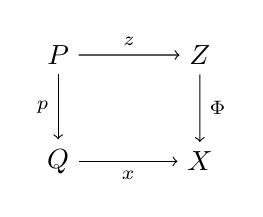
\begin{tikzpicture}[scale=1.5]
		\node (A) at (0,0.9) {$P$};
		\node (B) at (1.2,0.9) {$Z$};
		\node (C) at (0,0) {$Q$};
		\node (D) at (1.2,0) {$X$};
		\path[->,font=\scriptsize]
		(A) edge node[above]{$z$} (B)
		(B) edge node[right]{$\Phi$} (D)
		(C) edge node[below]{$x$} (D)
		(A) edge node[left]{$p$} (C);
	\end{tikzpicture}
	\end{center}
	with $p$ in $\PP$. As $Z$ is a colimit of a non-empty (because $R$ is non-empty) small diagram, then by $\PP$-accessibility, $\map{z}{P}{Z}$ factorizes as $[\pspan{P'}{X}{Y}{x'}{y'}]\circ p'$ for some $\pspan{P'}{X}{Y}{x'}{y'} \in R$ and $\map{p'}{P}{P'} \in \PP$. Then, by condition (d) of a strong path bisimulation, $\pspan{P}{X}{Y}{x'\circ p'}{y'\circ p'}$ belongs to $R$. Moreover, the following diagram commutes:
	\begin{center}
		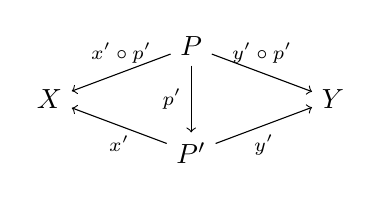
\begin{tikzpicture}[scale=1.5]
		\node (A) at (0,0.9) {$P$};
		\node (B) at (1.2,0.45) {$Y$};
		\node (D) at (-1.2,0.45) {$X$};
		\node (C) at (0,0) {$P'$};
		\path[->,font=\scriptsize]
		(C) edge node[below]{$x'$} (D)
		(A) edge node[above]{$x'\circ p'$} (D)
		(A) edge node[left]{$p'$} (C)
		(C) edge node[below]{$y'$} (B)
		(A) edge node[above]{$y'\circ p'$} (B);
	\end{tikzpicture}
	\end{center}
	Then, $z = [\pspan{P'}{X}{Y}{x'}{y'}]\circ p' = [\pspan{P}{X}{Y}{x'\circ p'}{y' \circ p'}]$.\\
	So, $x \circ p = \Phi \circ z = \Phi \circ [\pspan{P}{X}{Y}{x'\circ p'}{y' \circ p'}] = x'\circ p'$ by definition of $\Phi$. This means that we have the following commutative diagram:
		\begin{center}
		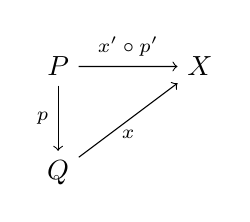
\begin{tikzpicture}[scale=1.5]
		\node (A) at (0,0.9) {$P$};
		\node (B) at (1.2,0.9) {$X$};
		\node (C) at (0,0) {$Q$};
		\path[->,font=\scriptsize]
		(A) edge node[left]{$p$} (C)
		(C) edge node[below]{$x$} (B)
		(A) edge node[above]{$x'\circ p'$} (B);
	\end{tikzpicture}
	\end{center}
	Then, by condition (b) of a strong path bisimulation, there is a path extension of $Y$:
	\begin{center}
		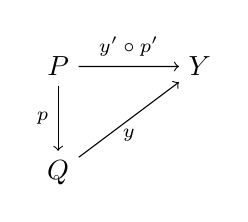
\begin{tikzpicture}[scale=1.5]
		\node (A) at (0,0.9) {$P$};
		\node (B) at (1.2,0.9) {$Y$};
		\node (C) at (0,0) {$Q$};
		\path[->,font=\scriptsize]
		(A) edge node[left]{$p$} (C)
		(C) edge node[below]{$y$} (B)
		(A) edge node[above]{$y'\circ p'$} (B);
	\end{tikzpicture}
	\end{center}
	such that $\pspan{Q}{X}{Y}{x}{y}$ belongs to $R$.\\
	Then the morphism $\map{\theta = [\pspan{Q}{X}{Y}{x}{y}]}{Q}{Z}$ is the lifting we were looking for:
		\begin{center}
	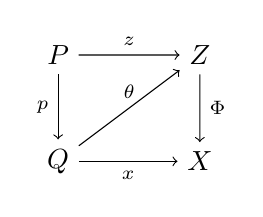
\begin{tikzpicture}[scale=1.5]
		\node (A) at (0,0.9) {$P$};
		\node (B) at (1.2,0.9) {$Z$};
		\node (C) at (0,0) {$Q$};
		\node (D) at (1.2,0) {$X$};
		\path[->,font=\scriptsize]
		(A) edge node[above]{$z$} (B)
		(B) edge node[right]{$\Phi$} (D)
		(C) edge node[below]{$x$} (D)
		(A) edge node[left]{$p$} (C)
		(C) edge node[above]{$\theta$} (B);
	\end{tikzpicture}
	\end{center}
So we deduce:

\begin{theo}
\label{the:equiv}
If $\M$ is $\PP$-accessible and if $X$ and $Y$ are strong path bisimilar then they are $\PP$-bisimilar.
\end{theo}





%%%%%%%%%%%%%%%%%%%%%%%%%%%%%%%%%
%%%%%%%%%%%%%%%%%%%%%%%%%%%%%%%%%%
%%%%%%%%%%%%%%%%%%%%%%%%%%%%%%%%%






\section{Presheaf models}
\label{preshmod}



Presheaf models were introduced in \cite{joyal96}, motivated by the work on pretopoi in \cite{joyal94}. We prove in this section that presheaf models are a particular case of accessible models.

Assume given a small category $\Delta$ with an initial object $J$. A \textbf{rooted presheaf on $\Delta$} is a functor $F$ from $\Delta^{op}$ to \textbf{Set} such that $F(J)$ is a singleton. Let $\presh{\Delta}_*$ be the category of rooted presheaves on $\Delta$ and natural transformations. We have a functor (called the \textbf{Yoneda embedding}) $\map{\yon}{\Delta}{\presh{\Delta}_*}$:
\begin{itemize}
\item[$\bullet$] we associate an object $P$ of $\Delta$ with the rooted presheaf $\yon(P)$ which maps:
\begin{itemize}
	\item every object $Q$ of $\Delta$ to $\Delta(Q,P)$,
	\item every morphism $\map{p}{Q}{Q'}$ of $\Delta$ to the function $\map{\yon(P)(p)}{\Delta(Q',P)}{\Delta(Q,P)} ~~~ f \mapsto f\circ p$.
\end{itemize}
\item[$\bullet$] we associate a morphism $\map{p}{P}{P'}$ with the natural transformation $\map{\yon(p)}{\yon(P)}{\yon(P')}$ defined by 
$$\map{\yon(p)_Q}{\Delta(Q,P)}{\Delta(Q,P')} ~~~~~ f \mapsto p\circ f$$
\end{itemize}

\begin{theo}
Let $\PP$ be the image of $\yon$ and $\M = \presh{\Delta}_*$. Then $\M$ is $\PP$-accessible.
\end{theo}

\begin{proof}~
		\begin{itemize}
			\item[$\star$] \textbf{$\PP$ is a full embedding of $\M$:} by the Yoneda lemma.
			\item[$\star$] \textbf{computation of colimits in $\M$:} consider a small diagram $\map{D}{U}{\M}$. The colimit in $\presh{\Delta}_*$ of $D$ is the colimit in $\presh{\Delta}$ (which is cocomplete \cite{borceux94b}) of the small (non-empty) diagram $\map{D_\bot}{U_\bot}{M}$ where:
				\begin{itemize}
					\item $U_\bot$ is the category obtained by adding an object $\bot$ to $U$ with a unique morphism from $\bot$ to any object of $U$ or $\bot$ and no morphism from an object of $U$ to $\bot$,
					\item $D_\bot$ maps $\bot$ to $\yon(J)$ (which is the initial object of $\M$ and $\PP$ by the Yoneda lemma), any object $u$ of $U$ to $D(u)$, the morphism from $\bot$ to $u$ object of $U_\bot$ to the unique natural transformation from $\yon(J)$ to $D_\bot(u)$ and any morphism $\nu$ of $U$ to $D(\nu)$.
				\end{itemize}
			\item[$\star$] \textbf{all trees exist:} consequence of the previous point.
			\item[$\star$] \textbf{$\PP$-accessibility:} let $\map{D}{U}{\PP}$ be a non-empty small diagram and $\map{f}{\yon(P)}{colim \ D}$ a morphism of $\M$ with $P$ in $\Delta$ and $colim \ D$ the colimit of $D$ in $\M$. $(colim \ D)(P)$ is computed as the quotient:
$$(\bigsqcup\limits_{u \in U} D(u)(P) \sqcup \Delta(P,J))/\sim$$
where $\sim$ is the equivalence relation on $\bigsqcup\limits_{u \in U} D(u)(P) \sqcup \Delta(P,J)$ generated by:
	\begin{itemize}
		\item for every $\map{\nu}{u}{u'}$ of $U$, for every $x \in D(u)(P)$, $x \sim D(\nu)_P(x)$,
		\item for every $x \in \Delta(P,J)$ and every $u$ in $U$, $x \sim \eta_u(x)$.
	\end{itemize}
	
Since $U$ is non-empty, every $x$ in $\Delta(P,J)$ is equivalent to some element of $\bigsqcup\limits_{u \in U} D(u)(P)$. So, every element of $(colim \ D)(P)$ is the image of one of the projections of an element of some $D(u)(P)$. Let $v$ be an object of $U$ and $x \in D(v)(P)$ such that $f_P(id_P) \in (colim \ D)(P)$ is the image of $x$ by the projection from $D(v)(P)$ to $(colim \ D)(P)$. By the Yoneda lemma, there exists a unique natural transformation $\map{\theta}{\yon(P)}{D(v)}$ such that $\theta_P(id_P) = x$. $\theta$ belongs to $\PP$ because $\PP$ is a full embedding of $\M$. If $\map{\pi_v}{D(v)}{colim \ D}$ is the morphism from the universal cocone, then by the Yoneda lemma, $f = \pi_v\circ\theta$.
		\end{itemize}
\end{proof}





%%%%%%%%%%%%%%%%%%%%%%%%%%%%%%%%%
%%%%%%%%%%%%%%%%%%%%%%%%%%%%%%%%%%
%%%%%%%%%%%%%%%%%%%%%%%%%%%%%%%%%


\section{Relationships with coreflections}
\label{relcoreflection}

We have seen in Chapter 1 that coreflections are a nice categorical way to express the fact that a computational model can be simulated by another one. This view was initiated in \cite{winskel84}, where it was shown in particular 
that event structures can be simulated by occurrence nets and so by 1-safe Petri nets. Note that the right adjoints of those coreflections give interesting constructions: in the case of occurrence nets in Petri nets, the right adjoint gives what is called the unfolding of a 1-safe Petri net. In this section, we prove that accessibility is preserved by coreflections.

In fact we can prove the even more general following theorem:

\begin{theo}
\label{the:core}
Let $\PP$ (resp. $\PP'$) be a subcategory of $\M$ (resp. $\M'$). Assume that:
\begin{itemize}
	\item[$\bullet$] $\M$ is $\PP$-accessible,
	\item[$\bullet$] there is a functor $\map{F}{\M}{\M'}$ such that:
	\begin{itemize}
		\item $F$ preserves trees, i.e., for every small diagram $\map{D}{U}{\PP}$, $F(colim \ D)$ is a colimit of $F\circ D$ in $\M'$,
		\item $F$ induces a functor from $\PP$ to $\PP'$,
		\item there is a functor $\map{G}{\PP'}{\PP}$ and a natural isomorphism $\map{\nu}{F\circ G}{id_{\PP'}}$.
	\end{itemize}
\end{itemize}
Then $\M'$ is $\PP'$-accessible.
\end{theo}


The preservation of trees holds for example when $F$ is a left adjoint. The other two conditions hold for example when $F$ induces a equivalence between $\PP$ and $\PP'$. So, we deduce:

\begin{coro}
If $\map{F}{\M}{\M'}$ is a coreflection, if $\PP'$ is the image of $\PP$ by $F$ and if $\M$ is $\PP$-accessible then $\M'$ is $\PP'$-accessible.
\end{coro}


\begin{proof}[Proof of Theorem \ref{the:core}] Let $\map{G}{\PP'}{\PP}$ and $\map{\nu}{F\circ G}{id_{\PP'}}$ a natural isomorphism.
\begin{itemize}
	\item[$\star$] \textbf{existence of trees:} let $\map{D}{U}{\PP'}$ be a small diagram. By preservation of trees and existence of trees in $\M$, $F(colim \ G\circ D)$ is a colimit of $F\circ G\circ D$ in $\M'$. But $\nu$ induces a natural isomorphism between $D$ and $F\circ G \circ D$. Then the colimit of $D$ in $\M'$ exists.
	\item[$\star$] \textbf{$\PP'$-accessibility:} Let $\map{z}{P'}{Z}$ morphism of $\M'$ with $P' \in \PP'$ and $(Z,(\eta_u)_{u\in U})$ is the colimit of a non-empty small diagram $\map{D}{U}{\PP'}$. 
	
	By naturality of $\nu$, the following diagram commutes:
	 \begin{center}
	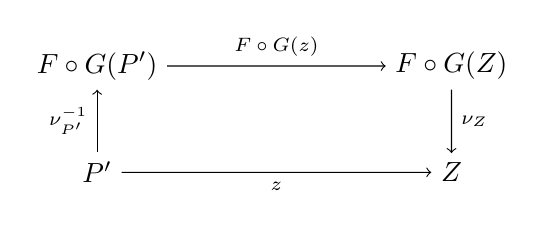
\begin{tikzpicture}[scale=1.5]
		%\node (A) at (4,2) {$colim \ D_{c'}$};
		\node (B) at (0,1) {$P'$};
		\node (C) at (3,1) {$Z$};
		\node (D) at (0,1.9) {$F\circ G(P')$};
		\node (E) at (3,1.9) {$F\circ G(Z)$};
		\path[->,font=\scriptsize]
		%(B) edge node[left]{$!$} (A)
		%(C) edge node[right]{$!$} (A)
		(B) edge node[below]{$z$} (C)
		(B) edge node[left]{$\nu_{P'}^{-1}$} (D)
		(E) edge node[right]{$\nu_{Z}$} (C)
		(D) edge node[above]{$F\circ G(z)$} (E);
	\end{tikzpicture}
	\end{center}
	
	By $\PP$-accessibility, $\map{G(z)}{G(P')}{G(colim \ D) = colim \ (G\circ D)}$ factorizes as $G(z) = \eta_u\circ p$ with $\map{p}{G(P')}{G\circ D(u)}$ morphism of $\PP$ and $\map{\eta_u}{G\circ D(u)}{colim(G \circ D)}$ is from the universal cocone. Then the following diagram commutes:
	 \begin{center}
	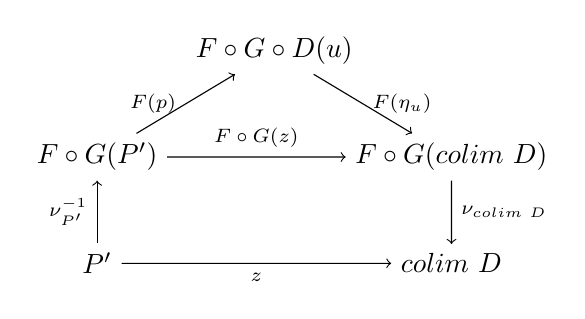
\begin{tikzpicture}[scale=1.5]
		\node (A) at (1.5,2.8) {$F\circ G \circ D(u)$};
		\node (B) at (0,1) {$P'$};
		\node (C) at (3,1) {$colim \ D$};
		\node (D) at (0,1.9) {$F\circ G(P')$};
		\node (E) at (3,1.9) {$F\circ G(colim \ D)$};
		\path[->,font=\scriptsize]
		(D) edge node[left]{$F(p)$} (A)
		(A) edge node[right]{$F(\eta_u)$} (E)
		(B) edge node[below]{$z$} (C)
		(B) edge node[left]{$\nu_{P'}^{-1}$} (D)
		(E) edge node[right]{$\nu_{colim \ D}$} (C)
		(D) edge node[above]{$F\circ G(z)$} (E);
	\end{tikzpicture}
	\end{center}
	
	
	Then $z$ factorizes as $\eta'_u\circ(\nu_{D(u)}\circ F(p)  \circ \nu_{P'}^{-1})$ with $\map{\eta'_u}{D(u)}{colim \ D}$ coming from the universal cocone and $\map{\nu_{D(u)}\circ F(p)  \circ \nu_{P'}^{-1}}{P'}{D(u)}$ morphism of $\PP'$.
\end{itemize}
\end{proof}






%%%%%%%%%%%%%%%%%%%%%%%%%%%%%%%%%
%%%%%%%%%%%%%%%%%%%%%%%%%%%%%%%%%%
%%%%%%%%%%%%%%%%%%%%%%%%%%%%%%%%%









\section{Unfoldings in accessible models}
\label{unfold}






\subsection{$\PP$-unfolding and bisimilarity}
\label{unfoldingandbisimilarity}


Remember that the unfolding of a transition system is an equivalent system without loops, obtained by ``unfolding'' the loops. More precisely, it is a tree which is bisimilar to the transition system. Concretely, the unfolding is defined as a transition system whose states are executions of the initial system, that is, it is defined as a glueing of all executions of this system. This is the way we will define more generally the unfolding in a categorical model.


%%%%%%%%%%%%%%%%%%%%%%%%%%%%%%




Let $\M$ a category where all trees exist and $X$ an object of $\M$. Let $\C_X$ be the small category whose:
\begin{itemize}
	\item objects are morphisms $\map{x}{P}{X}$ of $\M$ with $P$ in $\PP$,
	\item morphisms from $\map{x}{P}{X}$ to $\map{x'}{Q}{X}$ are morphisms $\map{p}{P}{Q}$ of $\PP$ such that the following diagram commutes:
	\begin{center}
		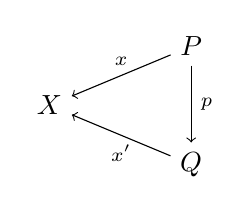
\begin{tikzpicture}[scale=1.5]
		\node (A) at (0,1) {$P$};
		\node (D) at (-1.2,0.5) {$X$};
		\node (C) at (0,0) {$Q$};
		\path[->,font=\scriptsize]
		(C) edge node[below]{$x'$} (D)
		(A) edge node[above]{$x$} (D)
		(A) edge node[right]{$p$} (C);
	\end{tikzpicture}
	\end{center}
\end{itemize}
We then define the small diagram $\map{F_X}{\C_X}{\PP}$  which maps every $\map{x}{P}{X}$ to $P$ and every $p$ to itself. Let $\text{Unfold}(X)$ be the colimit of $F_X$ in $\M$. We call it the \textbf{($\PP$-) unfolding of $X$}. Since $(X,(\map{x}{P}{X})_x)$ is a cocone of $F_X$, there is a unique morphism $\map{\text{unf}_X}{\text{Unfold}(X)}{X}$ such that for every $\map{x}{P}{X}$ with $P \in \PP$, the following diagram commutes:
	\begin{center}
		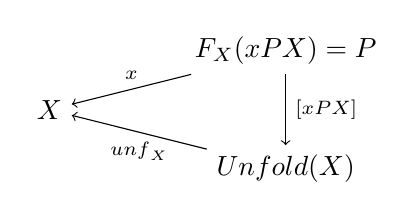
\begin{tikzpicture}[scale=1.5]
		\node (A) at (0,1) {$F_X(\map{x}{P}{X}) = P$};
		\node (D) at (-2,0.5) {$X$};
		\node (C) at (0,0) {$\text{Unfold}(X)$};
		\path[->,font=\scriptsize]
		(C) edge node[below]{$\text{unf}_X$} (D)
		(A) edge node[above]{$x$} (D)
		(A) edge node[right]{$[\map{x}{P}{X}]$} (C);
	\end{tikzpicture}
	\end{center}
where $[\map{x}{P}{X}]$ is the morphism coming from the colimit.

Using a similar argument to that in Theorem \ref{the:equiv}, we have the following:
\begin{theo}
When $\M$ is $\PP$-accessible, $\text{unf}_X$ is $\PP$-open and so $X$ and $\text{Unfold}(X)$ are $\PP$-bisimilar (strong path bisimilar).
\end{theo}

\begin{proof} Let a commutative diagram of the form :
\begin{center}
	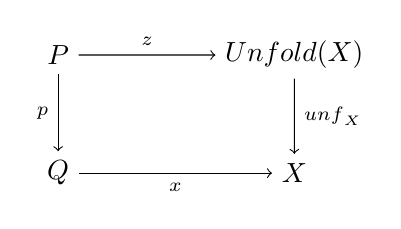
\begin{tikzpicture}[scale=1.5]
		\node (A) at (0,1) {$P$};
		\node (B) at (2,1) {$\text{Unfold}(X)$};
		\node (C) at (0,0) {$Q$};
		\node (D) at (2,0) {$X$};
		\path[->,font=\scriptsize]
		(A) edge node[above]{$z$} (B)
		(B) edge node[right]{$\text{unf}_X$} (D)
		(C) edge node[below]{$x$} (D)
		(A) edge node[left]{$p$} (C);
	\end{tikzpicture}
	\end{center}
	with $p \in \PP$. As $\text{Unfold}(X)$ is the colimit of a non-empty diagram (because there is a morphism from $I$ to $X$) in $\PP$, then by $\PP$-accessibility, there exist a morphism $\map{x'}{P'}{X}$ with $P'$ in $\PP$ and a morphism $\map{p'}{P}{P'}$ in $\PP$ such that $z = \nu_{x'}\circ p'$ where $\map{\nu_{x'}}{F_X(x') = P'}{\text{Unfold}(X)}$ is the morphism from the colimit. But, as $\text{Unfold}(X)$ together with the $\nu_x$ is a cocone of $F_X$, then $z = \nu_{x'}\circ p' = \nu_{x'\circ p'}$, and so by definition of $\text{unf}_X$, $x \circ p = \text{unf}_X\circ z = x' \circ p'$. Now consider $\map{\nu_x}{F_X(x) = Q}{\text{Unfold}(X)}$. Then :
	\begin{itemize}
		\item $\text{unf}_X\circ \nu_x = x$ by definition of $\text{unf}_X$
		\item $\nu_x \circ p = \nu_{x\circ p} = \nu_{x'\circ p'} = z$
	\end{itemize}
	i.e., the following diagram commutes :
	\begin{center}
	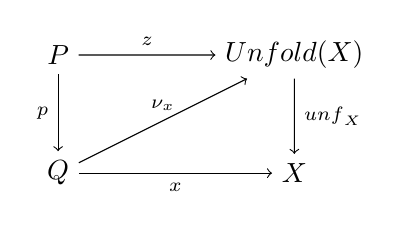
\begin{tikzpicture}[scale=1.5]
		\node (A) at (0,1) {$P$};
		\node (B) at (2,1) {$\text{Unfold}(X)$};
		\node (C) at (0,0) {$Q$};
		\node (D) at (2,0) {$X$};
		\path[->,font=\scriptsize]
		(A) edge node[above]{$z$} (B)
		(B) edge node[right]{$\text{unf}_X$} (D)
		(C) edge node[below]{$x$} (D)
		(A) edge node[left]{$p$} (C)
		(C) edge node[above]{$\nu_x$} (B);
	\end{tikzpicture}
	\end{center}
\end{proof}




%%%%%%%%%%%%%%%%%%%%%%%%%%%%%%

\subsection{Unfolding is a right adjoint}
\label{unfoldingrightadjoint}

The following lemma implies that the unfolding of a tree (and so of an unfolding) is isomorphic to the tree itself:

\begin{lemme}~
\begin{itemize}
	\item[(i)] When all trees exist in $\M$, $\text{Unfold}$ extends to a functor $\map{\text{Unfold}}{\M}{Tree(\M,\PP)}$.
	\item[(ii)] When $\M$ is $\PP$-accessible, $\PP$ is dense in $Tree(\M,\PP)$, i.e., for every $X \in Tree(\M,\PP)$, $(X,(x)_{\map{x}{P}{X}})$ is a colimit of $F_X$.
\end{itemize}
\end{lemme}

\begin{proof}~
\begin{itemize}
	\item[(i)] \begin{itemize}
			\item[$\star$] \textbf{definition of Unfold on morphisms:} let $\map{f}{X}{Y}$ be a morphism of $\M$. Then $(\text{Unfold}(Y),([\map{f\circ x}{P}{Y}])_{\map{x}{P}{X}})$ is a cocone of $F_X$. So there is a unique morphism $\map{\text{Unfold}(f)}{\text{Unfold}(X)}{\text{Unfold}(Y)}$ such that for every path $\map{x}{P}{X}$ of $X$, the following diagram commutes:
				\begin{center}
		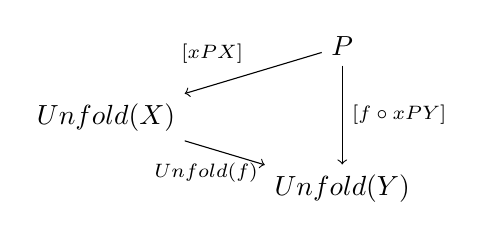
\begin{tikzpicture}[scale=1.2]
		\node (A) at (0,1.5) {$P$};
		\node (D) at (-2.5,0.75) {$\text{Unfold}(X)$};
		\node (C) at (0,0) {$\text{Unfold}(Y)$};
		\path[->,font=\scriptsize]
		(D) edge node[below]{$\text{Unfold}(f)~~~~~$} (C)
		(A) edge node[above]{$[\map{x}{P}{X}]~~~~~~~~~~~$} (D)
		(A) edge node[right]{$[\map{f\circ x}{P}{Y}]$} (C);
	\end{tikzpicture}
	\end{center}
	\item[$\star$] \textbf{identities:} we know that $id_{\textbf{Unfold(X)}}\circ \nu_x = \nu_x$ so by unicity, $\text{Unfold}(id_X) = id_{\text{Unfold}(X)}$.
	\item[$\star$] \textbf{compositions:} let $\map{f}{X}{Y}$ and $\map{g}{Y}{Z}$. By definition of Unfold, the following diagram commutes :
			\begin{center}
		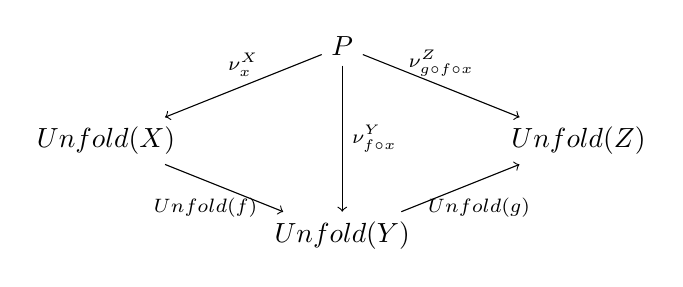
\begin{tikzpicture}[scale=1.2]
		\node (A) at (0,2) {$P$};
		\node (D) at (-2.5,1) {$\text{Unfold}(X)$};
		\node (C) at (0,0) {$\text{Unfold}(Y)$};
		\node (B) at (2.5,1) {$\text{Unfold}(Z)$};
		\path[->,font=\scriptsize]
		(D) edge node[below]{$\text{Unfold}(f)~~~~~$} (C)
		(A) edge node[above]{$\nu^X_x$} (D)
		(A) edge node[right]{$\nu^Y_{f\circ x}$} (C)
		(A) edge node[above]{$\nu^Z_{g\circ f \circ x}$} (B)
		(C) edge node[below]{$~~~~~\text{Unfold}(g)$} (B);
	\end{tikzpicture}
	\end{center}
	So by unicity, $\text{Unfold}(g\circ f) = \text{Unfold}(g) \circ \text{Unfold}(f)$.
	\end{itemize}
	\item[(ii)] \begin{itemize}
			\item[$\star$] \textbf{$(X,(x)_{\map{x}{P}{X}})$ is a cocone :} because the following diagram commutes :
			\begin{center}
		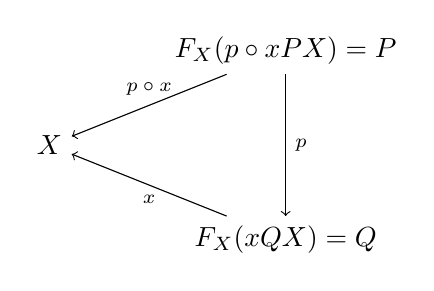
\begin{tikzpicture}[scale=1.2]
		\node (A) at (0,2) {$F_X(\map{p \circ x}{P}{X}) = P$};
		\node (D) at (-2.5,1) {$X$};
		\node (C) at (0,0) {$F_X(\map{x}{Q}{X}) = Q$};
		\path[->,font=\scriptsize]
		(C) edge node[below]{$x$} (D)
		(A) edge node[above]{$p\circ x$} (D)
		(A) edge node[right]{$p$} (C);
	\end{tikzpicture}
	\end{center}
			\item[$\star$] \textbf{colimit :} Give another cocone $(Z,(\map{\kappa_x}{P}{Z})_{\map{x}{P}{X}})$ of $F_X$.
				\begin{itemize}
					\item[$\bullet$] \textbf{construction of a morphism $\map{\Phi}{X}{Z}$ :} as $X$ is in $\tre{\M}{\PP}$, there is a small non-empty diagram $\map{G}{U}{\PP}$ such that $(X,(\mu_u)_{u \in U})$ is a colimit of $G$ for some $\mu_u$. So, for every $u$, $\map{\mu_u}{D(u)}{X}$ is an object of $\C_X$. Let us prove that $(Z,(\map{\kappa_{\mu_u}}{D(u)}{Z})_{u\in U})$ is a cocone of $D$, i.e., given a morphism $\map{\tau}{u}{v}$ in $U$, the following diagram commutes :
					\begin{center}
		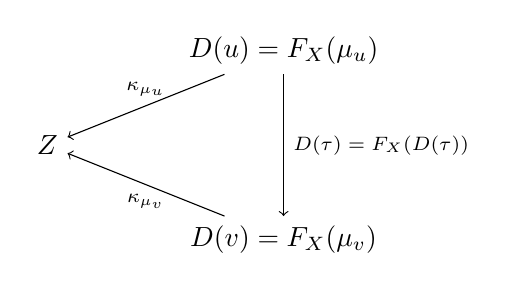
\begin{tikzpicture}[scale=1.2]
		\node (A) at (0,2) {$D(u) = F_X(\mu_u)$};
		\node (D) at (-2.5,1) {$Z$};
		\node (C) at (0,0) {$D(v) = F_X(\mu_v)$};
		\path[->,font=\scriptsize]
		(C) edge node[below]{$\kappa_{\mu_v}$} (D)
		(A) edge node[above]{$\kappa_{\mu_u}$} (D)
		(A) edge node[right]{$D(\tau) = F_X(D(\tau))$} (C);
	\end{tikzpicture}
	\end{center}
	which is true because $(Z,(\map{\kappa_x}{P}{Z})_{\map{x}{P}{X}})$ is a cocone of $F_X$. Then, there is a unique morphism $\map{\Phi}{X}{Z}$ such that for every $u \in U$, the following diagram commutes :
	\begin{center}
		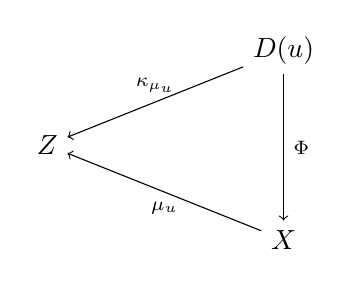
\begin{tikzpicture}[scale=1.2]
		\node (A) at (0,2) {$D(u)$};
		\node (D) at (-2.5,1) {$Z$};
		\node (C) at (0,0) {$X$};
		\path[->,font=\scriptsize]
		(C) edge node[below]{$\mu_u$} (D)
		(A) edge node[above]{$\kappa_{\mu_u}$} (D)
		(A) edge node[right]{$\Phi$} (C);
	\end{tikzpicture}
	\end{center}
					\item[$\bullet$] \textbf{$\Phi$ is a morphism of cocones from $(X,(x)_{\map{x}{P}{X}})$ to $(Z,(\map{\kappa_x}{P}{Z})_{\map{x}{P}{X}})$ :} i.e., for every $\map{x}{P}{X}$, $\Phi\circ x = \kappa_x$. As $X$ is the colimit of $D$ which is non-empty, then by $\PP$-accessibility, there is an object $u$ of $U$ and a morphism $\map{p}{P}{D(u)}$ in $\PP$ such that $x = \mu_u \circ p$. But, by the previous point, $\Phi\circ \mu_u = \kappa_{\mu_u}$ and as $(Z,(\map{\kappa_x}{P}{Z})_{\map{x}{P}{X}})$ is a cocone of $F_X$, $\kappa_{\mu_u}\circ p = \kappa_{\mu_u \circ p} = \kappa_x$. So, $\kappa_x = \Phi\circ \mu_u \circ p = \Phi\circ x$.
					\item[$\bullet$] \textbf{unicity of $\Phi$ :} any morphism of cocones from $(X,(x)_{\map{x}{P}{X}})$ to $(Z,(\map{\kappa_x}{P}{Z})_{\map{x}{P}{X}})$ is also a morphism of cocones from $(X,(\mu_u)_{u \in U})$ to $(Z,(\map{\kappa_{\mu_u}}{D(u)}{Z})_{u\in U})$ and so is equal to $\Phi$ by unicity.
				\end{itemize}
		\end{itemize}
\end{itemize}
\end{proof}

From this sort of density property, we deduce that the unfolding is a right adjoint of the inclusion of trees in $\M$. This result is similar to the one from \cite{winskel84} stating that the unfolding is the right adjoint of the inclusion of occurrence nets in 1-safe Petri nets.

\begin{theo}
When $\M$ is $\PP$-accessible, $\text{Unfold}$ is a right adjoint of $\map{\text{inj}}{\tre{\M}{\PP}}{\M}$, the embedding of $\tre{\M}{\PP}$ in $\M$. In particular, the injection of $\tre{\M}{\PP}$ in $\M$ is a coreflection.
\end{theo}

\begin{proof}~
\begin{itemize}
	\item[$\star$] \textbf{definition of the counit $\map{\epsilon}{\text{inj}\circ \text{Unfold}}{id_\M}$:} $\epsilon_X = \text{unf}_X$
	\item[$\star$] \textbf{naturality of $\epsilon$:} let $\map{f}{X}{Y}$ be a morphism of $\M$. We want to prove that $\text{unf}_Y\circ \text{Unfold}(f) = f \circ \text{unf}_X$. It is sufficient to prove that for every $\map{x}{P}{X}$, $\text{unf}_Y\circ \text{Unfold}(f)\circ\nu_x = f \circ \text{unf}_X\circ \nu_x^X$ :
	\begin{align*}
			f\circ \text{unf}_X \circ \nu_x 	&	=  f \circ x \\
      				 					&	=  \text{unf}_Y\circ \nu_{f\circ x}\\
									&	= \text{unf}_Y\circ \text{Unfold}(f) \circ \nu_x
		\end{align*}
	\item[$\star$] \textbf{definition of the unit $\map{\eta}{id_{\tre{\M}{\PP}}}{\text{Unfold}\circ \text{inj}}$ :} by density of $\PP$ in $\tre{\M}{\PP}$, for every $X \in \tre{\M}{\PP}$ there is a unique (iso)morphism $\map{\eta_X}{X}{\text{Unfold}(X)}$ such that for every $\map{x}{P}{X}$, $\eta_X\circ x = \nu_x$.
	\item[$\star$] \textbf{naturality of $\eta$:} let $\map{f}{X}{Y}$ be a morphism of $\tre{\M}{\PP}$. We want to prove that $\text{Unfold}(f)\circ\eta_X = \eta_Y\circ f$. It is sufficient to prove that for every $\map{x}{P}{X}$, $\text{Unfold}(f)\circ\eta_X\circ x = \eta_Y\circ f \circ x$ :
	\begin{align*}
			\text{Unfold}(f)\circ\eta_X\circ x 	&	=  \text{Unfold}(f)\circ \nu_x \\
      				 					&	=  \nu_{f\circ x}\\
									&	= \eta_Y\circ(f\circ x)
	\end{align*}
	\item[$\star$] \textbf{first equation of adjointness:} we want to prove that for every $X \in \tre{\M}{\PP}$, $\text{unf}_X\circ \eta_X = id_X$. By density, it is sufficient to prove that for every $\map{x}{P}{X}$, $\text{unf}_X\circ\eta_X \circ x = x$. This is true because $\text{unf}_X\circ \eta_X\circ x = \text{unf}_X \circ \nu_x = x$.
	\item[$\star$] \textbf{second equation of adjointness:} we want to prove that for every $X\in \M$, $\text{Unfold}(\text{unf}_X)\circ\eta_{\text{Unfold}(X)} = id_{\text{Unfold}(X)}$. It is sufficient to prove that for every $\map{x}{P}{X}$, $\text{Unfold}(\text{unf}_X)\circ \eta_{\text{Unfold}(X)}\circ \nu_x = \nu_x$. This is true because $\text{Unfold}(\text{unf}_X)\circ \eta_{\text{Unfold}(X)}\circ \nu_x = \text{Unfold}(\text{unf}_X) \circ \nu_{\nu_x} = \nu_{\text{unf}_X\circ \nu_x} = \nu_x$.
\end{itemize}
\end{proof}





%%%%%%%%%%%%%%%%%%
%%%%%%%%%%%%%%%%%%
%%%%%%%%%%%%%%%%%%



\section{Unfoldings and universal coverings}
\label{unicov}


Unfoldings and coverings of spaces \cite{may99} are very similar in the sense that they both ``unfold'' loops (or ``kill'' the first homotopy group). But it seems that there were no general formal links in the literature between those two structures. We present here a view toward this.



%%%%%%%%%%%%%%%%%%%%%%%%%
\subsection{Coverings of groupoids}
\label{groupoids}

Coverings of groupoids are more natural than coverings of spaces as they are defined by lifting properties and their existence does not assume any hypothesis on the groupoid. They are very close to coverings of spaces since a covering of a space induces a covering of its fundamental groupoid and lots of properties of coverings of spaces can be expressed on the induced coverings of groupoids \cite{may99}.

A \textbf{small pointed connected groupoid} (spc groupoids for short) is a pair $(\C,c)$ of a small connected groupoid $\C$ and an object $c$ of $\C$. A \textbf{pointed functor} is a functor $\map{F}{(\C,c)}{(\D,d)}$ between spc groupoids such that $F(c) = d$. We denote by $\grp$ the category of spc groupoids and pointed functors.

A \textbf{covering of a spc groupoids $(\C,c)$} is a pointed functor $\map{F}{(\tilde{\C},\tilde{c})}{(\C,c)}$ such that for every morphism $\map{f}{c}{c'}$ of $\C$ there exist a unique object $\tilde{c'}$ of $\tilde{\C}$ and an unique morphism $\map{\tilde{f}}{\tilde{c}}{\tilde{c'}}$ such that $F(\tilde{f}) = f$. We say that a covering is $\textbf{universal}$ if $\tilde{\C}(\tilde{c},\tilde{c}) = \{id_{\tilde{c}}\}$.

Covering are similar to open maps since they satisfy a lifting property. In fact, they are open maps when we consider the following subcategory of paths. Let $\I$ be the full subcategory of $\grp$ whose objects are the following two spc groupoids:
\begin{itemize}
	\item \textbf{0}, the spc groupoid with one object and only the identity as morphism,
	\item \textbf{1}, the spc groupoid with two objects: 
	\begin{center}
	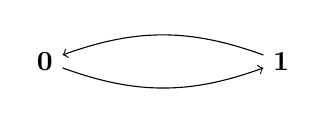
\begin{tikzpicture}
		\node (0) at (0,0) {\textbf{0}};
		\node (1) at (3,0) {\textbf{1}};
		\draw[->] (0) to [bend right = 20] (1);
		\draw[->] (1) to [bend right = 20] (0);
	\end{tikzpicture}
	\end{center}
	pointed on 0.
\end{itemize}
It is easy to check that $\grp$ is $\I$-accessible.

Coverings are exactly the open maps whose lifts are unique. Universal coverings are universal in the category of coverings in the following sense \cite{may99}: given a universal covering $\map{F}{(\tilde{\C},\tilde{c})}{(\C,c)}$ and a covering $\map{G}{(\D,d)}{(\C,c)}$, then there is a unique pointed functor $\map{H}{(\tilde{\C},\tilde{c})}{(\D,d)}$ such that $G\circ H = F$. Moreover, $H$ is a covering. This means that universal covering is initial in the category of coverings. In particular, universal coverings are unique up to isomorphism. Contrary to universal coverings of spaces, universal coverings of groupoids always exist \cite{may99}. 




%%%%%%%%%%%%%%%%%%%%%%%%%%%%%%%%%
\subsection{Unfoldings and unique path lifting property}
\label{uniquepathlifting}

We have just seen that (universal) coverings are defined by unique lifting property. Now let us see the link between unfoldings and unique liftings.

We say that a morphism $\map{f}{X}{Y}$ is a \textbf{$(\PP$-) covering} if it has the \textbf{unique path lifting property}, i.e., if for every commutative diagram:
	\begin{center}
	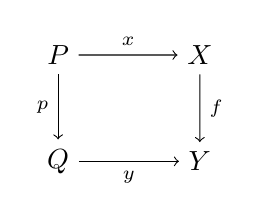
\begin{tikzpicture}[scale=1.5]
		\node (A) at (0,0.9) {$P$};
		\node (B) at (1.2,0.9) {$X$};
		\node (C) at (0,0) {$Q$};
		\node (D) at (1.2,0) {$Y$};
		\path[->,font=\scriptsize]
		(A) edge node[above]{$x$} (B)
		(B) edge node[right]{$f$} (D)
		(C) edge node[below]{$y$} (D)
		(A) edge node[left]{$p$} (C);
	\end{tikzpicture}
	\end{center}
	with $\map{p}{P}{Q} \in \PP$, there exists a unique morphism $\map{\theta}{Q}{X}$ such that the following diagram commutes:
	\begin{center}
	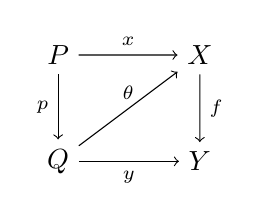
\begin{tikzpicture}[scale=1.5]
		\node (A) at (0,0.9) {$P$};
		\node (B) at (1.2,0.9) {$X$};
		\node (C) at (0,0) {$Q$};
		\node (D) at (1.2,0) {$Y$};
		\path[->,font=\scriptsize]
		(A) edge node[above]{$x$} (B)
		(B) edge node[right]{$f$} (D)
		(C) edge node[below]{$y$} (D)
		(A) edge node[left]{$p$} (C)
		(C) edge node[above]{$\theta$} (B);
	\end{tikzpicture}
	\end{center}
This is the same as $\PP$-open but with the unicity of the lift. 

The following result states that unfolding is a covering and that moreover it is initial among coverings.

\begin{theo} When $\M$ is $\PP$-accessible:
\begin{itemize}
	\item[i)] $\text{unf}_X$ has the unique path lifting property
	\item[ii)] for every morphism $\map{f}{Y}{X}$ which has the unique lifting property, there is a unique morphism $\map{\tilde{f}}{\text{Unfold}(X)}{Y}$ such that $f\circ\tilde{f} = \text{unf}_X$. Moreover, $\tilde{f}$ has the unique path lifting property.
\end{itemize}
\end{theo}

\begin{proof}~
\begin{itemize}
	\item[i)] This is a consequence of ii) because $id_X$ has the unique path lifting property and $id_X\circ \text{unf}_X = \text{unf}_X$ and so $\text{unf}_X = \widetilde{id_X}$.
	\item[ii)] 
		\begin{itemize}
			\item[$\star$]\textbf{construction of $\tilde{f}$:} for every $\map{x}{P}{X}$ path of $X$, by the unique path lifting property, there is a unique $\map{\tilde{x}}{P}{Y}$ such that:
			\begin{center}
	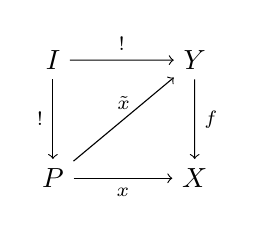
\begin{tikzpicture}[scale=1.5]
		\node (A) at (0,1) {$I$};
		\node (B) at (1.2,1) {$Y$};
		\node (C) at (0,0) {$P$};
		\node (D) at (1.2,0) {$X$};
		\path[->,font=\scriptsize]
		(A) edge node[above]{$!$} (B)
		(B) edge node[right]{$f$} (D)
		(C) edge node[below]{$x$} (D)
		(A) edge node[left]{$!$} (C)
		(C) edge node[above]{$\tilde{x}$} (B);
	\end{tikzpicture}
	\end{center}
	i.e., a unique $\tilde{x}$ such that $f\circ \tilde{x} = x$. Let us prove that $(Y,(\tilde{x})_{\map{x}{P}{X}})$ is a cocone of $F_X$, i.e., if $\map{p}{P}{Q} \in \PP$ and $\map{x}{Q}{X}$, we have to prove that $\widetilde{x\circ p} = \tilde{x}\circ p$. But, $f\circ \widetilde{x\circ p} = x \circ p = (f\circ \tilde{x}) \circ p = f \circ (\tilde{x} \circ p)$. So, by unicity, $\widetilde{x\circ p} = \tilde{x}\circ p$. Now, as $(\text{Unfold}(X),(\nu_x)_x)$ is a colimit of $F_X$, there is a unique $\map{\tilde{f}}{\text{Unfold}(X)}{Y}$ such that for every $\map{x}{P}{X}$, $\tilde{f}\circ \nu_x = \tilde{x}$ and so, $f\circ \tilde{f} \circ \nu_x = f\circ \tilde{x} = x = \text{unf}_X \circ \nu_x$ and by unicity, $f\circ \tilde{f} = \text{unf}_X$.
			\item[$\star$] \textbf{unicity of $\tilde{f}$:} let $\map{g}{\text{Unfold}(X)}{Y}$ such that $f\circ g = \text{unf}_X$. Then, for every $\map{x}{P}{X}$, $f\circ g \circ \nu_x = \text{unf}_X\circ \nu_x = x$. Then, by unicity of $\tilde{x}$, $g\circ \nu_x = \tilde{x}$ and unicity of the definition of $\tilde{f}$, $g = \tilde{f}$.
			\item[$\star$] \textbf{existence of the lift:} Let a diagram of the form :
			\begin{center}
	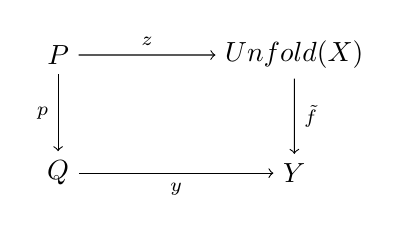
\begin{tikzpicture}[scale=1.5]
		\node (A) at (0,1) {$P$};
		\node (B) at (2,1) {$\text{Unfold}(X)$};
		\node (C) at (0,0) {$Q$};
		\node (D) at (2,0) {$Y$};
		\path[->,font=\scriptsize]
		(A) edge node[above]{$z$} (B)
		(B) edge node[right]{$\tilde{f}$} (D)
		(C) edge node[below]{$y$} (D)
		(A) edge node[left]{$p$} (C);
		%(C) edge node[above]{$\theta$} (B);
	\end{tikzpicture}
	\end{center}
	with $p \in \PP$. Then, we have the following commutative diagram :
	\begin{center}
	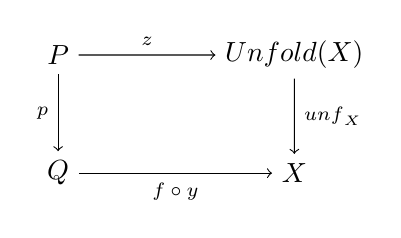
\begin{tikzpicture}[scale=1.5]
		\node (A) at (0,1) {$P$};
		\node (B) at (2,1) {$\text{Unfold}(X)$};
		\node (C) at (0,0) {$Q$};
		\node (D) at (2,0) {$X$};
		\path[->,font=\scriptsize]
		(A) edge node[above]{$z$} (B)
		(B) edge node[right]{$\text{unf}_X$} (D)
		(C) edge node[below]{$f\circ y$} (D)
		(A) edge node[left]{$p$} (C);
		%(C) edge node[above]{$\theta$} (B);
	\end{tikzpicture}
	\end{center}
	As $\text{unf}_X$ is $\PP$-open, there is $\map{\theta}{Q}{\text{Unfold}(X)}$ such that:
	\begin{center}
	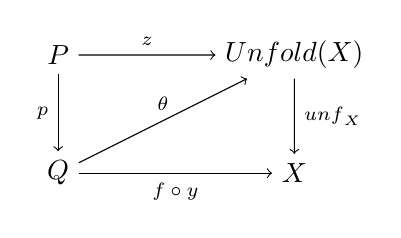
\begin{tikzpicture}[scale=1.5]
		\node (A) at (0,1) {$P$};
		\node (B) at (2,1) {$\text{Unfold}(X)$};
		\node (C) at (0,0) {$Q$};
		\node (D) at (2,0) {$X$};
		\path[->,font=\scriptsize]
		(A) edge node[above]{$z$} (B)
		(B) edge node[right]{$\text{unf}_X$} (D)
		(C) edge node[below]{$f\circ y$} (D)
		(A) edge node[left]{$p$} (C)
		(C) edge node[above]{$\theta$} (B);
	\end{tikzpicture}
	\end{center}
	Now, $f\circ \tilde{f}\circ \theta = \text{unf}_X \circ \theta = f \circ y$ and so $\tilde{f}\circ \theta = \widetilde{\text{unf}_X\circ\theta} = y$ and so 			
	\begin{center}
	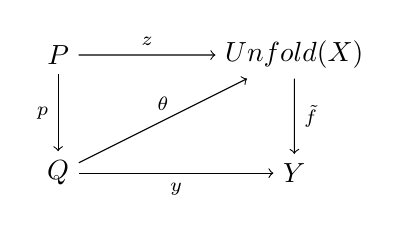
\begin{tikzpicture}[scale=1.5]
		\node (A) at (0,1) {$P$};
		\node (B) at (2,1) {$\text{Unfold}(X)$};
		\node (C) at (0,0) {$Q$};
		\node (D) at (2,0) {$Y$};
		\path[->,font=\scriptsize]
		(A) edge node[above]{$z$} (B)
		(B) edge node[right]{$\tilde{f}$} (D)
		(C) edge node[below]{$y$} (D)
		(A) edge node[left]{$p$} (C)
		(C) edge node[above]{$\theta$} (B);
	\end{tikzpicture}
	\end{center}
			\item[$\star$] \textbf{unicity of the lift:} assume that we have two lifts:
			\begin{center}
	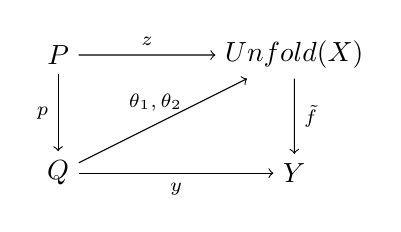
\begin{tikzpicture}[scale=1.5]
		\node (A) at (0,1) {$P$};
		\node (B) at (2,1) {$\text{Unfold}(X)$};
		\node (C) at (0,0) {$Q$};
		\node (D) at (2,0) {$Y$};
		\path[->,font=\scriptsize]
		(A) edge node[above]{$z$} (B)
		(B) edge node[right]{$\tilde{f}$} (D)
		(C) edge node[below]{$y$} (D)
		(A) edge node[left]{$p$} (C)
		(C) edge node[above]{$\theta_1,\theta_2~~$} (B);
	\end{tikzpicture}
	\end{center}
	By $\PP$-accessibility, we know that every path of $\text{Unfold}(X)$ is of the form $\map{\nu_{x_i}}{P}{\text{Unfold}(X)}$, for some $x_i$. Then, the previous diagram is of the form :
	\begin{center}
	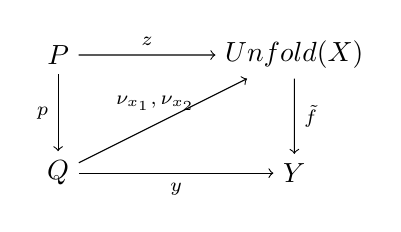
\begin{tikzpicture}[scale=1.5]
		\node (A) at (0,1) {$P$};
		\node (B) at (2,1) {$\text{Unfold}(X)$};
		\node (C) at (0,0) {$Q$};
		\node (D) at (2,0) {$Y$};
		\path[->,font=\scriptsize]
		(A) edge node[above]{$z$} (B)
		(B) edge node[right]{$\tilde{f}$} (D)
		(C) edge node[below]{$y$} (D)
		(A) edge node[left]{$p$} (C)
		(C) edge node[above]{$\nu_{x_1},\nu_{x_2}~~$} (B);
	\end{tikzpicture}
	\end{center}
	with $x_1 = f\circ\tilde{x_1} = f\circ\tilde{f}\circ \nu_{x_1} = f\circ y = f\circ\tilde{f}\circ \nu_{x_2} = f\circ\tilde{x_2} = x_2$
		\end{itemize}
\end{itemize}
\end{proof}

In the case of $\grp$ and $\I$, this implies that the unfolding is a covering and is initial in the category of coverings. So we deduce:

\begin{coro} The universal covering of a spc groupoid coincides with its $\I$-unfolding.\end{coro}


\section*{Conclusion}

In this chapter, we have describe a general class of models for which bisimilarity of Joyal et al. is equivalent to the existence of a relation on executions, paths of the systems. These models are those from which we have a nice subcategory of trees constructed as colimits of path shapes or executions forms. In those models, we have also proved that we have a nice notion of unfolding, which is right adjoint to the inclusion of trees and that it is a universal covering, that is, initial among coverings, morphisms having the unique lifting property. In particular, we have describe an explicit relation between universal covering of a groupoid in algebraic topology and a unfolding.





